%\documentclass[aps,prb]{revtex4}
%\documentclass[aps,prb,twocolumn]{revtex4-1}
\documentclass[showpacs,aps,prb,reprint,superscriptaddress]{revtex4-1}
%\documentclass[showpacs,aps,prl,reprint,superscriptaddress,showkeys,floatfix,citeautoscript]{revtex4-1}
\usepackage{bm}
\usepackage{graphicx}
\usepackage{graphics}
\usepackage{amsmath,amssymb,amstext}
\usepackage{amsfonts}

\usepackage{epstopdf}
\usepackage{hyperref}
\usepackage{hyperref}
\hypersetup{
    colorlinks,%
    citecolor=blue,%
    linkcolor=blue,%
    urlcolor=blue
}
%\usepackage{pgf}
\usepackage{tikz}\usetikzlibrary{petri}
%\usepackage{bbold}
%\usepackage{makeidx}
\newcommand{\TS}[1]{{$\rightarrow$ {\sl#1}}}
\newcommand{\LUIS}[1]{\textcolor{blue}{\fbox{Luis} {\sl#1}}}
\newcommand{\Jesus}[1]{\textcolor{red}{\fbox{Jesus} {\sl#1}}}
\begin{document}


\newcommand{\be}   {\begin{equation}}
\newcommand{\ee}   {\end{equation}}
\newcommand{\ba}   {\begin{eqnarray}}
\newcommand{\ea}   {\end{eqnarray}}
\newcommand{\ve}  {\varepsilon}

\newcommand{\nhat}{\hat{n}}
\newcommand{\veck}{\textbf{k}}
\newcommand\ep{\epsilon}
\newcommand\g{\gamma}
\newcommand\s{\sigma}
\newcommand\up{\uparrow}
\newcommand\dw{\downarrow}
\newcommand\down{\downarrow}
\newcommand{\ed}[1]{\ep_{d#1}}
\newcommand{\ket}[1]{\vert #1 \rangle}
\newcommand{\ann}{a^{\dagger}}
\newcommand{\dann}{d^{\dagger}}
\newcommand{\tdots}{t_{dots}}
\newcommand{\gammaA}[1]{\gamma_{A,#1}}
\newcommand{\gammaB}[1]{\gamma_{B,#1}}
\newcommand{\GreenG}[2]{G_{#1}^{ #2} (\omega) }
%\newcommand{\bra}[3]{\langle {#3} \vert}

\newcommand{\super}{\vert \Delta \vert}





%%%%%%%%%%%%%%%%%%%%%%%%%%%%%%%%%%%%%%%%%%%%%%%%%%%%%%%%%%%%%%%%%%%%%%%%%%%%%%%
\title{ Majorana-Kondo coexistance in a double quantum dot. }

\author{Jesus D. Cifuentes}
\affiliation{Instituto de F\'{\i}sica, Universidade de S\~{a}o Paulo,
C.P.\ 66318, 05315--970 S\~{a}o Paulo, SP, Brazil}
\author{Luis G.~G.~V. Dias da Silva}
\affiliation{Instituto de F\'{\i}sica, Universidade de S\~{a}o Paulo,
C.P.\ 66318, 05315--970 S\~{a}o Paulo, SP, Brazil}

\date{ \today }

\begin{abstract}

(To be written)


\end{abstract} 
%\pacs{ APS does not use it anymore}
%\keywords{Quantum Spin-Hall effect, Edge transport, Topological insulators}

\maketitle


%%%%%%%%%%%%%%%%%%%%%%%%%%%%%%%%%%%%%%%%%%%%%%%%%%%%%%%%%%%%%%%%%%%%%%%%%%%%%%%
\section{Introduction}
\label{sec:Intro}

In the last few decades the interest in the so called Majorana fermions has been growing rapidly. The particle proposed by the physicist Ettore Majorana  as the real field solution of the Dirac equation describes a fermion which is its own antiparticle, hence it has no charge nor mass. To the date no fundamental particle with these characteristics has been found. However,  theoretical research predicts that Majorana Fermions emerge as quasi-particles at the boundary of certain topological superconductors . Recently, the new technological innovations have allowed the observation of Majorana signatures in different topological materials \citep{mourik_signatures_2012,das_zero-bias_2012,deng_anomalous_2012,zhang_quantized_2018} . 

Despite the positive experimental results, the existence of  Majorana   Fermions is still not fully demonstrated. One of the reasons  is that some of the main Majorana properties have not been measured. In particular, the majorana fermions are predicted to satisfy non-abelian statistics. This property is of especial interest due to its promising applications in topological quantum computing. The braiding protocol based on  Majorana's non-abelian statistics is the key to  fault-tolerant quantum gates \cite{sarma_majorana_2015}. 

Experimental proposals for braiding measurements have been  proposed  in one dimensional majorana chains.  The system inspired in the famous Kitaev toy model is a promising example of these topological superconductors.  The chain emulates a spinless p-wave superconducting wire. With the adequate combination of magnetic field,  superconducting gap and Rashba spin-orbit coupling  the wire enters into a topological phase in which zero-mode majorana bound states emerge. 

A promising method to detect majorana modes consists in attaching a Quantum Dot (QD) to the edges of a majorana chain in the topological phase and executing transport measurements through the QD \cite{liu_detecting_2011} . The majorana mode at the end of the chain then leaks inside the QD \cite{vernek_subtle_2014} which produces a zero-bias conductance peak of half a quanta $\frac{e^{2}}{2h}$ through the dot. This is a majorana signature which produces half of the expected peak by a regular fermion.  Recently, experiments including hybrid Majorana-QD systems have been performed \cite{deng_majorana_2016} . In addition, the similarity of this phenomenon with the Kondo effect, where the zero-bias conductance peak takes  $\frac{e^{2}}{h}$, motivated the study of combined Kondo-Majorana physics in this system \cite{lee_kondo_2013,ruiz-tijerina_interaction_2015}. The study revealed that the non  \\


%following the prescription by \citet{oreg_helical_2010} and \citet{lutchyn_majorana_2010}.   

% Despite the positive experimental results, the proof One of the most promising aplications of Majorana Fermions is the implementaition of  braiding procedures  which are the key to implement fault-tolerant quantum computers. 
% Most of the experiments have been based on tunneling spectroscopy in junctions between TS and non metallic (NM) leads, where resonances have been observed at zero energy, consistent with the presence of Majorana zero\textendash energy modes. A downside of the tunneling spectroscopy technique  is that it probes not only the end of the Topological Superconductor(TS), but its bulk as well ,
% which completely destroys the qubit information. A less destroying



% In addition, the use of QDs favors the manipulation of the majorana mode through the shifting of the dot gate voltage and the hopping parameters.
 One of the insights of this method is that the information of the qubit is not completely destroyed as in other methods like tunneling spectroscopy. 
 
 When majoranas are connected to multidot systems it is possible to manipulate the majorana mode inside the QDs  by tuning the gate voltage and  tunnel couplings. This fa
 
 
 The other advantage  is the possibility of “moving” around Majoranas  in multidot systems by shifting the QD gate voltages and Hence the approach is suitable for the implementation of braiding procedures . The simplest system where Majorana manipulation is possible is  a  Double Quantum Dot (DQD) coupled to a majorana chain. By tuning the QD gate voltages and the majorana coupling we will be able to probe the mobility of the majorana modes through the dots. 
 
 When both dots are coupled to the leads the Double Quantum Dot exhibits an antiferromagnetic interaction known as  Ruderman-Kittel-Kasuya-Yosida (RKKY) interaction\cite{ruderman_indirect_1954,kasuya_theory_1956,yosida_magnetic_1957}. On the other hand, when only one QD is coupled to the leads and the other Dot is attached to the QD,  the Kondo effect is annihilated due to the destructive interference  generated by extra dot \cite{dias_da_silva_transmission_2008}. Our study includes how the Majorana mode interacts with these two effects.  





% Then the majorana  as proposed by  \citet{liu_detecting_2011} and consists in coupling a quantum dot (QD) to the end of a TS. The analysis performed by Liu of this model revealed a  when the TS is in the topological phase,  which a signature of
% Majorana physics. On 2014, \citet{vernek_subtle_2014} showed that the Majorana Bound State at the end of the TS actually leaks inside the QD , which produces the conductance decay. and the model has been based for braiding experimental proposals.










% To the date experimental procedures have been put forward. ery recently the first evidence of Majorana end states
% in TS has been found in multiple experiments


% as quasi-particles in certain types of topological materials have increased. The Majoranas are fermions that are their own anti-particle, hence have no charge nor mass. 
% The majorana is predicted to be one of the most suitable alternatives to implement fault-tolerant quantum computers. Many experiments showing majorana signatures in the conductivity have been performed. 





% Basics of Majorana Bound states:  zero-energy edge states in 1D topological superconductors.  

% Discovery on semiconductor nanowires \cite{Oreg:Phys.Rev.Lett.:177002:2010,Lutchyn:Phys.Rev.Lett.:77001:2010,Alicea:Reports:2012} etc. Experimental results \cite{Mourik:Science:1003:2012} \LUIS{Add others.}


% Leaking of Majorana to a QD: \cite{vernek_subtle_2014}, Interplay of Kondo and Majorana\cite{ruiz-tijerina_interaction_2015} Important results: Majorana and Kondo co-exist in the quantum dot even if the dot is non-topological.

% More recent experimental results: Deng et al. \cite{deng_majorana_2016} attached a QD to the end of a nanowire.

% Here we study the coupling of a MBS to a \emph{double} quantum dot system. 

% \TS{Punchline} Multidot systems offer the possiblity of ``moving'' Majoranas aroung using gate voltages and couplings. ossibility of Majorana braiding. Here, we study the simplest case, which is a double dot system.

%%%%%%%%%%%%%%%%%%%%%%%%%%%%%%%%%%%%%%%%%%%%%%%%%%%%%%%%%%%%%%%%%%%%%%%%%%%%%%%
\section{Model and methods}
\label{sec:modelmethods}

%\LUIS{Jesus, put the description of the system and the Hamiltonian here. Put a schematic figure of the DQD setup as well}




We consider the setup shown in Figure \ref{fig:GenModel} in which a Majorana Bound State (MBS) at the edge of Topological Superconductor(TS) is coupled to a double quantum dot (DQD), which is attached to a single metallic lead. The Hamiltonian of this system can be partitioned in four terms: the DQD Hamiltonian $H_{DQD}$ , the Lead Hamiltonian $H_{Lead}$ , the DQD-lead interaction  $H_{DQD-Lead}$ and the coupling between the DQD and the Majorana mode $H_{M-DQDs}$ and   

\begin{equation}
H=H_{DQD}+H_{Lead}+H_{DQD-Lead}+H_{M-DQD} 
\label{eq:Model}
\end{equation}


%-----------F I G U R E  1 ------
\begin{figure}[bt]
\begin{center}
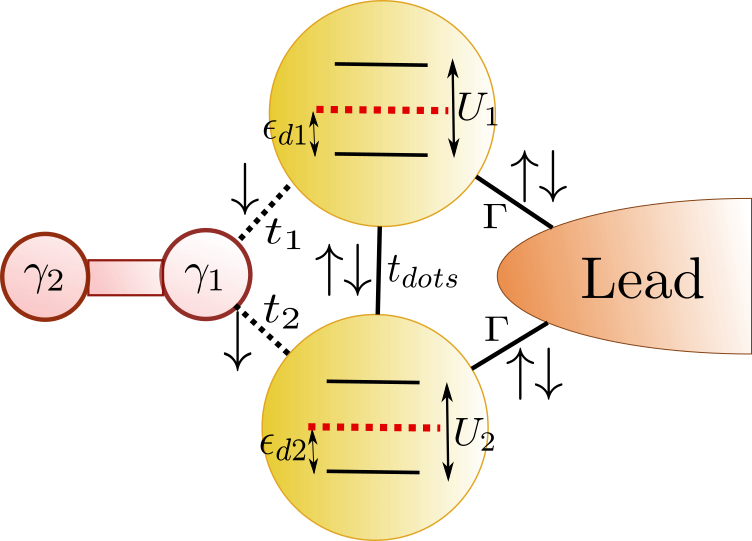
\includegraphics[scale=0.4]{Graficos/Model.png}
\caption{ DQD-Majorana set-up. Solid lines: standard coupling. Dashed lines: majorana spin-$\dw$ effective couplings \eqref{eq:H_MDQD}. The atomic energy levels appear inside each QD. Red dashed lines represent the Fermi level.  
}
%
\label{fig:GenModel}
\end{center}
\end{figure}
%-----------E N D  F I G U R E  1 ------


The interacting Anderson Model describes the DQD-lead system  
%d_{i\sigma}^{\dagger}d_{i\sigma}
\begin{align}
\begin{split}
    H_{DQD}=&  \sum_{i\in\{1,2\}} \sum_{\sigma\in \{ \dw , \up\}}  \left(\epsilon_{di}+\frac{U_i}{2}\right)\hat{n}_{i\sigma}+ \frac{U_i}{2}(\sum_{\sigma} \hat{n}_{i\sigma}-1)^{2} \\ 
&\ \ \ \ \ + \sum_{\sigma \in \{\up , \dw\}} \tdots(\dann_{1\sigma}  d_{2\sigma}+\dann_{2\sigma}  d_{1\sigma}), \label{eq:H_DQD}
\end{split}
\end{align}

and 
\begin{eqnarray}
H_{Lead} & = & \sum_{\mathbf{k}\sigma }\epsilon_{\mathbf{k}}c_{\mathbf{k}\sigma }^{\dagger}c_{\mathbf{k}\sigma } \label{eq:H_L}\\ 
H_{DQD-Lead} & = &  \sum_{\mathbf{k}\sigma }\sum_{i\in\{1,2\}}V_{i\textbf{k}} c_{\mathbf{k}\sigma }^{\dagger}d_{i\sigma}+V^*_{i\textbf{k}} d_{i\sigma}^{\dagger}c_{\mathbf{k}\sigma }  \label{eq:H_DQDL},
\end{eqnarray}
%
where $\ed{i}$ is the energy level of Dot $i$, $U_i$ is the Coulomb repulsion and $\tdots$ is the coupling parameter between both QDs. The operator $\dann_{i\sigma}$ creates a particle in Dot $i$ with spin $\sigma$ and $\hat{n}_{i\sigma}:=d_{i\sigma}^{\dagger}d_{i\sigma}$ is the particle number operator of state $i$.  $c_{\mathbf{k}\sigma }^{\dagger}$ is the creation operator a particle with momentum $\mathbf{k}$ and spin
$\sigma$ in the lead.  $\epsilon_{\mathbf{k}l}$ is the corresponding energy
 and $V_i(\textbf{k})$ describes the tunneling coupling between the lead and Dot $i$ . \\

% To model the interaction between the DQD and the Majorana Mode we define the majorana operators as the

The majorana modes are modeled as a superposition of the creation and annihilation operators of a spin $\dw$ particle $f_\dw$
\begin{equation}
    \gamma_1 := \frac{1}{\sqrt{2}} \left( f^\dagger_{\dw} + f_{\dw}\ \right) , \gamma_2 := \frac{i}{\sqrt{2}} \left( f^\dagger_{\dw} - f_{\dw} \right). \label{eq:MajOp}
\end{equation}


This makes possible to define an effective coupling between the Majorana Mode and the DQD by attaching $\gamma_1$ with the spin-$\dw$ channel in the QDs

%H_{TS} & = & 2\epsilon_{m}\gamma_{1}\gamma_{2}\nonumber \\
\begin{eqnarray}
H_{M-DQD} & = &  \sum_{i=1}^2t_{i} \left(d_{i\downarrow}^{\dagger}\gamma_{1}+\gamma_{1}d_{i\downarrow}\right) + \epsilon_M \gamma_1\gamma_2. 
% \\
% & = &  \sum_{i}t_{i} \left(d_{i\downarrow}^{\dagger}f^\dagger_{\dw} + 
% f_{\downarrow}d_{i\dw} +d_{i\downarrow}^{\dagger}f_{\dw}+
% +f_{\downarrow}^{\dagger} d_{i\downarrow}\right).
\label{eq:H_MDQD}
\end{eqnarray}
where $t_i$ is the coupling parameter between the majorana mode and QD $i$. $\epsilon_m$ is the coupling energy between both majorana modes.  




% \begin{equation}
%     \omega\Green{A,B}&=\delta_{A^{\dagger},B}+\Green{\left[A,H\right],B}
% \end{equation}

% \Jesus{Should I put the other terms? }


\citeauthor{ruiz-tijerina_interaction_2015}  showed that this effective coupling  is able to reproduce effectively the results obtained when the Kitaev chain in the topological phase is attached to a single QD.  \\
 
% ---------------------------------------------------
\subsection{Methods}
With ballistic transport we found the Green function associated to the first dot  $\Green{d_1d^\dagger_1}$  to be 



associated to
\begin{equation}
    \rho_{i\sigma}(\omega)= \frac{-i}{\pi}\mathcal{I}\left[ \mathcal{G}^R_{i\sigma}(\omega) \right],
    \label{eq:SpectralFunction}
\end{equation}



In order to calculate the properties of the model given by Eq.\ (\ref{eq:Majorana-ham}), we used the Numerical Renormalization Group (NRG) approach. \cite{wilson_renormalization_1975,sindel_numerical_2005,bulla_numerical_2008} 
 To to improve the efficiency of the code we used the symmetries of the system.  Now, one of the insights of this model is that spin-$\dw$ particle number $\hat{N_\dw}$ is not preserved due to the term $(d_{i\downarrow}^{\dagger}f^\dagger_{\dw} + 
f_{\downarrow}d_{i\dw})$ in $H_{M-DQD}$ \eqref{eq:Majorana-ham}. However the  spin-$\up$ particle number $\hat{N}_\up$ and the parity of spin-$\dw$ particles $\hat{P}_\dw = \pm $ ($+$ even, $-$ odd) are still conserved. \\

To implement the NRG code it is necessary to define a cut-off energy $D$ \cite{bulla_numerical_2008}. By convention, we define this energy to be double the coulomb repulsion of the first dot $D = 2U_1$. For convenience we use $D$ as energy unit.  \\



The local density of states (LDOS) on each dot is obtained by computing the spectral function 


%
where $\mathcal{G}^R(\omega)$ is the Fourier transform of the Green function $\mathcal{G}^R(t,T)=-i\theta(t) \langle \{d_{i,\sigma}(t) , d_{i,\sigma}^\dagger(0)\} \rangle$. The spectral functions were calculated with the DM-NRG method.\cite{hofstetter_generalized_2000} 



\Jesus{Luis... should I put details about the methods that we used?. Till now, I just mentioned them with references. }
\LUIS{It is fine for now}
%(NRG) method [44–46]: one can refer Ref. 47 for a review.
%For better efficiency, we exploit the symmetries that our sys-
%tem has: [Q ↑ , H] = [P ↓ , H] = 0 where Q ↑ and P ↓ are
%charge number operator for spin-↑ electrons and parity op-
%erator for the sum Q ↓ of spin-↓ electrons and f electrons, re-
%spectively. Note that the QD-MFS hopping changes Q ↓ by
%even numbers only. For the
%we calculate the spec-where |ni is
%the many-body eigenstate with energy E n and |0i is th






\Jesus{The analysis that I did explains the energy scale where the majorana peaks appear. But I don't know if it is good to do the base change that is the way we used to explain the Kondo satellites. }

\LUIS{No need to change the basis. But can you add some dashed lines in the plots of Fig. 3 showing these values as a reference? }

% It is now suitable to do change to the basis of symmetric ($d_+$) and anti-symmetric ($d_-$) states 
% \[
%   d_{+ , \sigma} = \frac{1}{\sqrt{2}} (d_{1\sigma} +d_{2\sigma}) \ , \ 
%   d_{- , \sigma} = \frac{1}{\sqrt{2}} (d_{1\sigma} -d_{2\sigma}),
% \]



% where Hamiltonian \eqref{eq:AtomicHam}  looks like 
% \begin{align}
% H = \sum_{\sigma}  \frac{U}{4}\left( \left( \hat{N}-2 \right)^2- \hat{E}^2 \right) + \frac{t}{\sqrt{2}} (\gamma_1 d_{+,\dw}+d^\dagger_{+,\dw}\gamma_1 ).
% \label{eq:ExchangeHam}
% \end{align}


% where  $\hat{N} = \sum_\sigma (\hat{n}_{+,\sigma} + \hat{n}_{-,\sigma})$ is the total particle number and $\hat{E} = \sum_\sigma (d^\dagger_{+,\sigma}d_{-,\sigma} + d^\dagger_{-,\sigma}d_{+,\sigma})$ is a term representing the state exchange between $+$ and $-$ spaces. An schematic representation of this interaction is observed in Figure \ref{fig:ExchangeModel}.



% %-----------F I G U R E  2 ------
% \begin{figure}[tb]
% \begin{center}
% 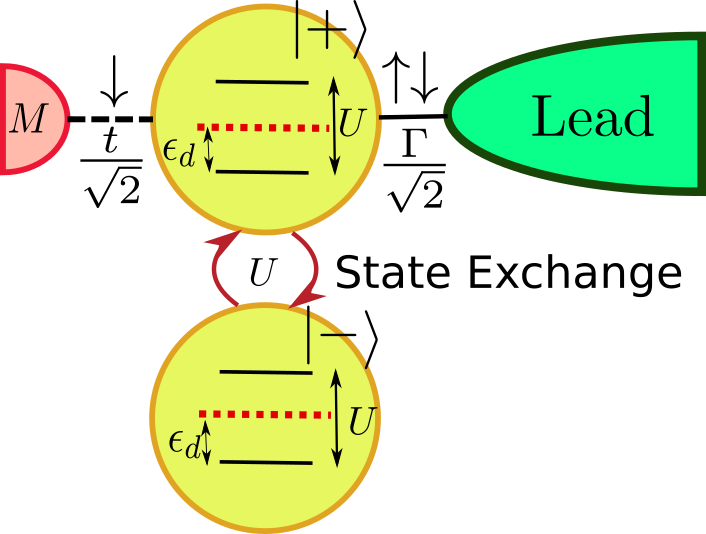
\includegraphics[scale=0.35]{Graficos/ExchangeMod.png}
% \caption{ Schematic representation of Hamiltonian \eqref{eq:ExchangeHam} After the base-change, only the symmetric state $ d^\dagger_+$ is coupled to Majorana mode. The majorana coupling is cut to $\frac{t}{2}$ and there appears an exchange term between the symmetric and the $ d^\dagger_+$ and the $ d^\dagger_-$ anti-symmetric state. 
% }
% %
% \label{fig:ExchangeModel}
% \end{center}
% \end{figure}
% %-----------E N D  F I G U R E  2 ------








%Using the symmetries of the system , $\hat{N}_\up$ and $P_\dw$ conservation, we can divide it into blocks of size $4\times4$. 




\section{NRG Results}
\label{sec:Results}

%---------------------t1=t2----------------------------------------------

\subsection{Connecting the Majorana Mode \label{sub:t1=t2}}

\textbf{Parameters:}

    $\Gamma \sim 2.83\times10^{-2}D,\  t_{dots}=0 ,\  U_{1,2} = -2\ed{1,2} = 0.5D.$

\textbf{Variable:}
    $$t_1=t_2 \in [0\  ,\  2\times10^{-2}D].$$
%----------------------FIGURE 2--------------------------------
    \begin{figure}[bt]
    \centering
    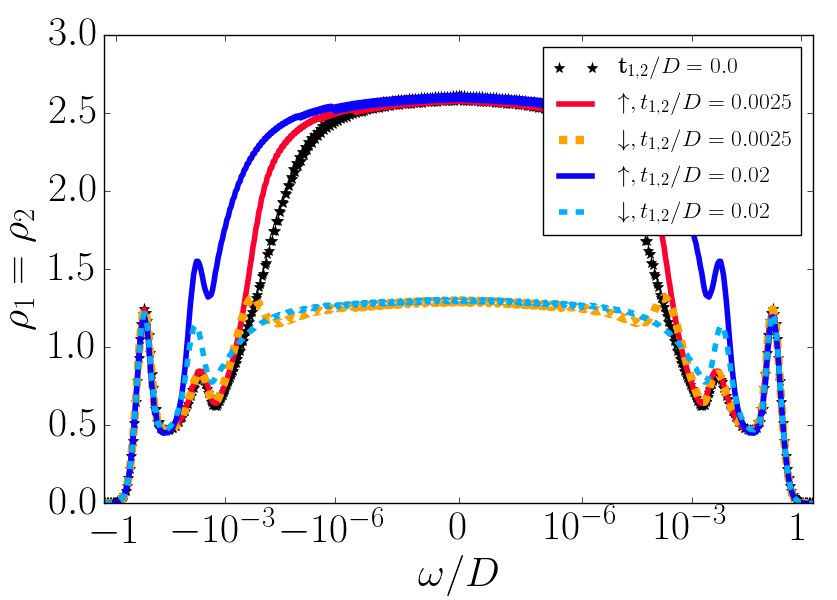
\includegraphics[scale=0.35]{Graficos/LogPlot.png}
    \caption{\label{fig:t1=t2/logplot} Density of states at each QD of the horizontal dashed cuts in Figure \ref{fig:t1=t2-2D} . The energy is in logarithmic scale. At the Fermi energy $(\omega =0)$ the spin-$\up$ DOS is $\rho_\up(0) \sim \frac{1}{4\pi\Gamma}$. At $t_{1,2}=0$ $\rho_up=\rho_\dw$. However, for  $t>0$  $\rho_\dw(0) = \frac{\rho_\up(0)}{2}$ which is a majorana signature. The spin-$\up$ and spin-$\dw$ DOS split at an energy scale that depends on the parameter $t_{1}=t_2$.}
    \end{figure}
%------------------------------------------------------


    
The first process consists in attaching the Majorana mode to both Quantum Dots symmetrically. For this, we scale up the coupling parameter $t_1=t_2$ from $0D$ (Decoupled) to $0.02D$ (Completely coupled). The other parameters where chosen with an equilibrium between the dot energy and Coulomb repulsion $(\ed{1,2}=-\frac{U_{1,2}}{2})$  and  without inter-dot coupling $t_{dots}=0$. These circumstances guarantee that the system preserves Particle Hole Symmetry (PHS). Thus the Density of States (DOS) of particles and holes remains equal at all instances $(\rho(-\omega) = \rho(\omega))$. \\
    
For $t_1 =t_2 = 0$ the system consists only of a DQD coupled to a NM lead. Since the model is symmetric for both QDs , the Kondo density of states  splits between both dots (See Figure \ref{fig:t1=t2/logplot}). Apart from the coulomb peaks that appear at $\omega=0.25D=\pm \ed{1,2}$, two new sided peaks emerge at low-energies $(\omega \sim 10^{-2}D)$. These peaks are the result of the of a strong anti-ferromagnetic interaction between both dots caused by the indirect exchange of quantum states through the Lead. This interaction receives the name of Ruderman-Kittel-Kasuya-Yosida (RKKY) interaction\cite{ruderman_indirect_1954,kasuya_theory_1956,yosida_magnetic_1957}. \\
    
    

Once the MZM is attached $t_1 =t_2 > 0$ the spin-$\up$ and spin-$\dw$ DOS split at low energies. In both dots the spin-$\dw$ DOS at the Fermi energy ($\omega =0$) decays to the half of the spin-$\up$ DOS $\rho_\dw = \frac{\rho_\up}{2} $. It was previously verified  by  \citeauthor{ruiz-tijerina_interaction_2015} that the Majorana signature of a QD in the Kondo regime coupled to a TS wire is the half-decay of the spin-$\dw$ DOS. Hence the results from Figure \ref{fig:t1=t2/logplot} imply that the majorana signature appears in both dots. \\
    
Moreover, there is an additional effect caused by the indirect exchange between the QDs through the Majorana mode. The energy scale of this effect was computed for the atomic limit in equation \eqref{eq:displacement}. Depending on this energy scale the consequences the indirect exchange through the majorana mode will produce different results.

%The consequences of this effect depend on the energy range of the majorana couplings $t_1=t_2$.
    
\begin{enumerate}
    \item If $t_1=t_2 \ll \Gamma $ two more satellites are formed at very low energies only in the spin-$\dw$ DOS. These peaks correspond to the displacement energy $\frac{4t^2}{U}$ found in the atomic limit \eqref{eq:displacement}  (See Figure \ref{fig:t1=t2-2D} Spin-down $\omega \sim 10^{-3}D$ ). 
    \item For $t_1=t_2 \sim \Gamma$ the Majorana peaks do not appear in the spin-$\dw$ DOS any more. Instead, we observe a combined Kondo-majorana physics in the satellite peaks. This produces an increase of the DOS at the energy scale where the satellite peaks appeared at $t_1=t_2=0$. Since $\rho_\up$ must double $\rho_\dw$ at $\omega=0$, the spin-$\up$ satellites are greater (See  \ref{fig:t1=t2/logplot} for $t_{1,2}=0.02D$). This effect causes the rapid scale-up of satellite peaks for $t_1=t_2>0.01D$  (See \ref{fig:t1=t2-2D} Spin-$\up$, $\omega \sim 10^{-2}D$).
    
\end{enumerate}
    
    \Jesus{Maybe we should include a plot comparing the temperature of Kondo and majorana physics.}

    \begin{figure}[bt]
        \begin{center}
            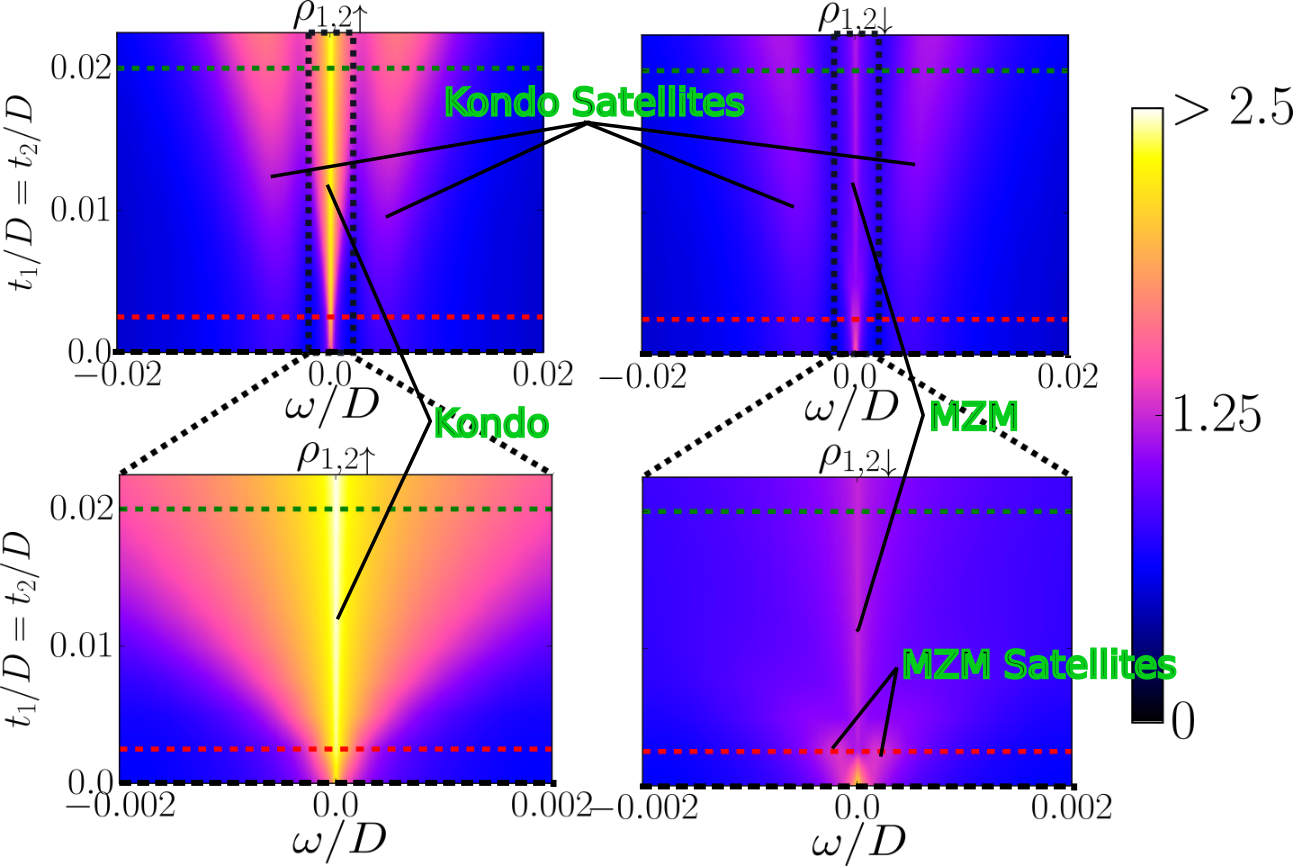
\includegraphics[scale=0.26]{Graficos/t1=t2-2D.png}
            \caption{\label{fig:t1=t2-2D}Evolution of the DOS of both QDs through $t_1 = t_2$ tuning. UP: Energy scale $\omega \sim 10^{-2}D$. DOWN: Energy scale $\omega \sim 10^{-3}D$. LEFT: Spin $\up$. RIGHT: Spin $\dw$. \LUIS{IN the paper plot you need to remove to comments ``MZM satellites'', etc. We can add small arrows and explain in the main text.}}
            \end{center}
    \end{figure}
    
%-----------------------------e2------------------------------------------    
\subsection{Transferring the MZM \label{sec:e2}}

\textbf{Parameters:}

\begin{align*}
    \Gamma \sim 2.83*10^{-2}D, t_{dots}= & 0 , U_{1,2} = -2\ed{1} = 0.5 \\
    t_1=t_2=&0.02D
\end{align*}
\textbf{Variable:}
$$\ed{2} \in [-0.25D \  , -0.05D]$$

This process starts in the final state of \ref{sub:t1=t2} with the DQD coupled symmetrically to the Majorana mode and $t_1=t_2=0.02D$. The idea of this process is to break PHS by increasing the energy of the second QD $\ed{2}$. This procedure should induce the Majorana to tunnel only into the first dot. \\


\begin{figure}[bt]
\centering
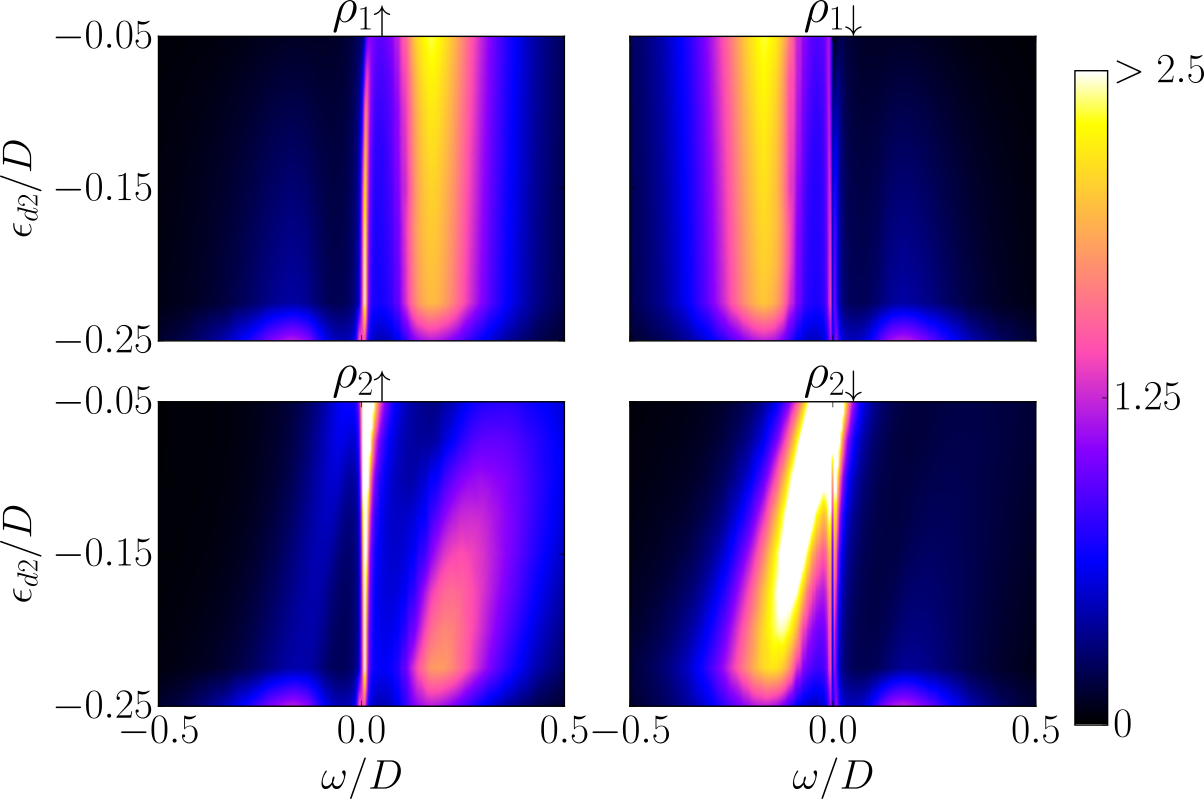
\includegraphics[scale=0.3]{Graficos/2Dhigh.png}
\caption{\label{fig:2D/Shift_ed2} Evolution of the DOS of both QDs through the $\ed{2}$ tuning. UP: QD1. DOWN: QD2. LEFT: Spin $\up$. RIGHT: Spin $\dw$.}
\end{figure}


In \ref{fig:2D/Shift_ed2} we observe that both, the Kondo and the MZM peaks are preserved in the first QD as well as the majorana signature (See \ref{fig:ed2/Fermi}) when $\ed{2}$ is scaled up to $-0.1$.  However,  PHS breaking will favor the growth of the spin-$\up$ hole $(w>0)$  satellite and the spin-$\dw$ particle $(w<0)$ satellite.


\begin{figure}[bt]
\centering
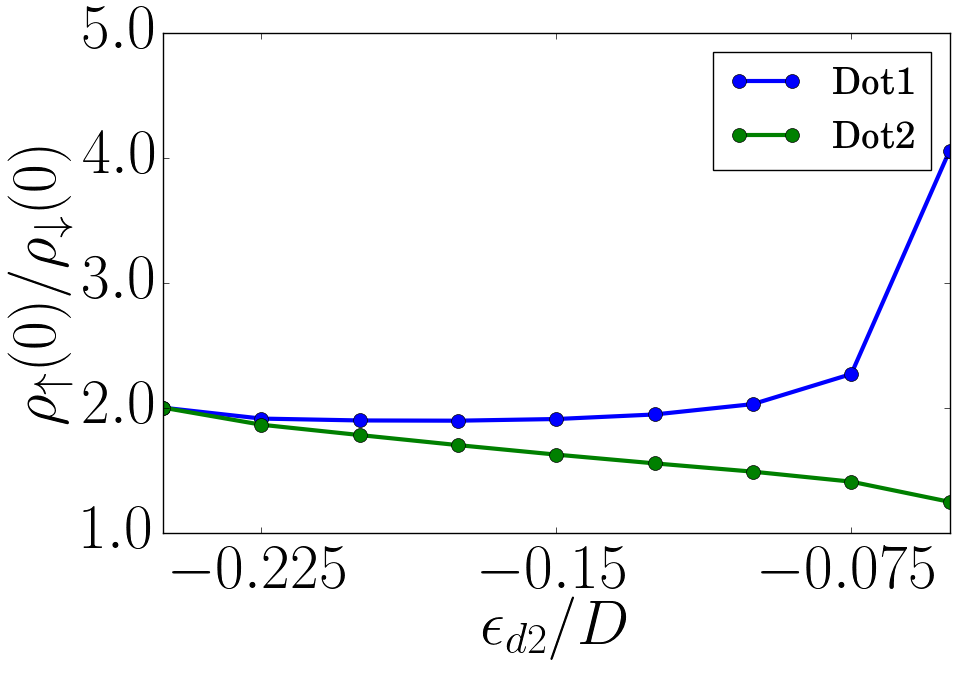
\includegraphics[scale=0.3]{Graficos/e2-Fermi.png}
\caption{\label{fig:ed2/Fermi} As described in \ref{sub:t1=t2} the relation $\frac{\rho_\up(0)}{\rho_\up(0)}=2$ determines the Majorana Signature . This picture shows the evolution of the relation $\frac{\rho_\up(0)}{\rho_\up(0)}$ for both QDs. While QD2 losses rapidly the Majorana signature, QD1 maintains it till $\ed{2}\sim -0.1D$. For  $\ed{2}>-0.1D$ the coulomb peaks in QD2 overlap with the fermi energy which destroys the Kondo effect in the first dot (See Figure \ref{fig:2D/Shift_ed2}). }

\end{figure}



%---------------------------------------------------------------------------

%---------------------------------------------------------------------------





    
\section{Concluding remarks}
\label{sec:Conclusions}

Conclusion goes here.

\begin{acknowledgments}
The authors thank Edson Vernek for enlightening discussions.  L.G.G.V.D.S. acknowledges financial support by CNPq (grants No. 307107/2013-2 and 449148/2014-9), and FAPESP (grant No. 2016/18495-4).
\end{acknowledgments}

\LUIS{Only ONE bib file}

%---------------------- Apendix A------------------------


%-----------------------------------------------------------

%\bibliographystyle{unsrtnat}
%\addcontentsline{toc}{section}{\textbf{References}}
\bibliography{Majorana_DQD}

 \appendix
 
 
\begin{widetext}
\begin{equation}
    \GreenG{d_{1\downarrow},d_{1\downarrow}^{\dagger}}{\MDQD}=\left[\left(\GreenG{d_{1\downarrow},d_{1\downarrow}^{\dagger}}{\GDQD } \right)^{-1}+\frac{\omega}{\omega+\epsilon_{M}}\frac{E_{d_{1\dw}f_{\dw}}^{\MDQD}}{\left[\GreenG{f_{\downarrow},f_{\downarrow}^{\dagger}}{\MDQD-d_{1}}\right]^{-1}}\right]^{-1}.
\end{equation}
where 
\begin{equation}
    E_{d_{1\dw}f_{\dw}}^{\MDQD}=\left(t_{1}+t_{2}\frac{\left(t_{dots}+\sum_{\mathbf{k}}\frac{V_{1}V_{2}^{*}}{\omega-\epsilon_{\mathbf{k}}}\right)}{\omega-\epsilon_{2}-\sum_{\mathbf{k}}\frac{V_{2}V_{2}^{*}}{\omega-\epsilon_{\mathbf{k}}}}\right)\left(t_{1}^{*}+t_{2}^{*}\frac{\left(t_{dots}^{*}+\sum_{\mathbf{k}}\frac{V_{1}^{*}V_{2}}{\omega-\epsilon_{\mathbf{k}}}\right)}{\omega-\epsilon_{2}-\sum_{\mathbf{k}}\frac{V_{2}^{*}V_{2}}{\omega-\epsilon_{\mathbf{k}}}}\right).
\end{equation}
\Jesus{This fact is difficult to explain. I will need more plots and writing the appendix. For now I will leave here some results}

We then need to compute $\GreenG{f_{\downarrow},f_{\downarrow}^{\dagger}}{\MDQD-d_{1}}$ . This graph is much simple. The neighborhood of  $f_{\downarrow}$ in graph ${\MDQD-d_{1}}$ are $d_2$ (above) and the inverted DQD(bellow). These neighbors are disconnected, hence we can include the in the green function independently. The term above is simply the dot $d_{2\downarrow}$ connected with the lead . 
\begin{equation}
    \frac{\frac{\omega}{\omega+\epsilon_{M}}\left\Vert t_{2}\right\Vert ^{2}}{\omega-\epsilon_{2}-\sum_{\mathbf{k}}\frac{V_{2}V_{2}^{*}}{\omega-\epsilon_{\mathbf{k}}}}.
\end{equation}

 
The term generated by the connection of $f_{\downarrow}$  with the inverted $DQD$ is a bit more complicated. First we need to include the term given by the connection with  $d_{2\downarrow}^\dagger$ which is 

The other term is the contact with the DQD which can be expressed as 
\begin{equation}
    \GreenG{f_{\downarrow},f_{\downarrow}^{\dagger}}{\MDQD-d_{1}}=\left[\omega-\epsilon_{M}-\frac{\frac{\omega}{\omega+\epsilon_{M}}\left\Vert t_{2}\right\Vert ^{2}}{\omega-\epsilon_{2}-\sum_{\mathbf{k}}\frac{V_{2}V_{2}^{*}}{\omega-\epsilon_{\mathbf{k}}}}-\frac{\frac{\omega}{\omega+\epsilon_{M}}\left\Vert t_{2}\right\Vert ^{2}}{\omega+\epsilon_{2}-\sum_{\mathbf{k}}\frac{V_{2}V_{2}^{*}}{\omega+\epsilon_{\mathbf{k}}}}-\frac{\omega}{\omega+\epsilon_{M}}\frac{E_{f_{\dw}d_{1\dw}^\dagger}^{\MDQD-d_1}}{\left[\GreenG{d_{1\downarrow}^{\dagger},d_{1\downarrow}{\dagger}}{\MDQD-d_{1}-f_{\downarrow}}\right]^{-1}}\right]^{-1}.
\end{equation}
Now, note that that graph $\MDQD-d_{1}-f_{\downarrow}$ is actually a double quantum dot with negated couplings. Hence 
\end{widetext}


\end{document}



% \section{Atomic limit: Change of basis}
% Returning to Hamiltonian \eqref{eq:AtomicHam} the change of basis is given by 
% \[
%   d_{+ , \sigma} = \frac{1}{\sqrt{2}} (d_{1\sigma} +d_{2\sigma}) \ , \ 
%   d_{- , \sigma} = \frac{1}{\sqrt{2}} (d_{1\sigma} -d_{2\sigma}).
% \]

% These new operators satisfy the fermionic anti-commutation relations 
%  \[ \{d_{\pm , \sigma}, d^\dagger_{\pm , \sigma}\} = 1 , \{ d_{\pm , \sigma}, d^\dagger_{\mp , \sigma}\} = 0,
% \]
%  so that the may be considered as fermion operators. All lineal terms in \eqref{eq:AtomicHam} are trivially adapted to the new base. The repulsion potential 
% $$\sum_{i} (\sum_{\sigma} d_{i \sigma}^{\dagger}d_{i \sigma}-1)^{2} = (\sum_{\sigma} d_{1 \sigma}^{\dagger}d_{1 \sigma}-1)^{2} + (\sum_{\sigma} d_{2 \sigma}^{\dagger}d_{2 \sigma}-1)^{2} . $$ 
% gives rise to a non-trivial interaction between the new states. To find this interaction we define the particle number operator  
% \[\hat{n}_{i,\sigma}:= d^\dagger_{i,\sigma}d_{i,\sigma}.\] 

% So that 
% \begin{align}
% \hat{n}_{1,\sigma}= & \frac{1}{2} \left( \hat{n}_{+,\sigma} + \hat{n}_{-,\sigma} + d^\dagger_{+,\sigma}d_{-,\sigma} + d^\dagger_{-,\sigma}d_{+,\sigma} \right) \\
% = & \frac{1}{2} \left( \hat{N}_\sigma + \hat{E}_\sigma \right),
% \end{align}
% with $\hat{N}_\sigma = \hat{n}_{+,\sigma} + \hat{n}_{-,\sigma}$ and $\hat{E}_\sigma = d^\dagger_{+,\sigma}d_{-,\sigma} + d^\dagger_{-,\sigma}d_{+,\sigma}. $ Similarly 

% \[\hat{n}_{2,\sigma}= \frac{1}{2} \left( \hat{N}_\sigma - \hat{E}_\sigma \right).  \]
% Hence 
% \begin{align}
% \sum_{i} (\sum_{\sigma} d_{i \sigma}^{\dagger}d_{i \sigma}-1)^{2} = & \left(\frac{\hat{N} +\hat{E}}{2}-1 \right) ^{2} + \left( \frac{\hat{N} -\hat{E}}{2}-1 \right)^{2} \\
%  = & \frac{\left( \hat{N}-2 \right)^2- \hat{E}^2}{2},
% \end{align}

% with $\hat{N}_\sigma=\sum_\sigma \hat{N}_\sigma $ , $\hat{E}=\sum_\sigma \hat{E}_\sigma $. Note that opeator $\hat{N}$ represents the total occupation number inside both dots. If this occupation is different than $2$ there is an imbalance between particles and dots that is punished by this term. The term $E^2$ is much more interesting since this one is the responsible for the emergence of satellite peaks in the DOS. To understand what it makes it is simple to observe its results when applied to a based ordered by $\vert + , - \rangle$. 
% \[ \hat{E}^2 \vert \up , 0 \rangle =  \hat{E} \vert 0 , \up \rangle = \vert \up , 0 \rangle   \] 
% \[ \hat{E}^2 \vert \up , \dw \rangle =  \hat{E} \left( \vert 0 , \up\!\dw \rangle + \vert \up\!\dw , 0 \rangle \right) = 2\vert \up , \dw \rangle - 2\vert \dw , \up \rangle  \]

% \begin{align}
% H = \sum_{\sigma}  \frac{U}{4}\left( \left( \hat{N}-2 \right)^2- \hat{E}^2 \right) + \frac{t}{\sqrt{2}} (\gamma_1 d_{+,\dw}+d^\dagger_{+,\dw}\gamma_1 )
% \label{t+}
% \end{align}